% Options for packages loaded elsewhere
\PassOptionsToPackage{unicode}{hyperref}
\PassOptionsToPackage{hyphens}{url}
%
\documentclass[
  12pt,
]{article}
\usepackage{amsmath,amssymb}
\usepackage{lmodern}
\usepackage{ifxetex,ifluatex}
\ifnum 0\ifxetex 1\fi\ifluatex 1\fi=0 % if pdftex
  \usepackage[T1]{fontenc}
  \usepackage[utf8]{inputenc}
  \usepackage{textcomp} % provide euro and other symbols
\else % if luatex or xetex
  \usepackage{unicode-math}
  \defaultfontfeatures{Scale=MatchLowercase}
  \defaultfontfeatures[\rmfamily]{Ligatures=TeX,Scale=1}
  \setmainfont[]{Times New Roman}
\fi
% Use upquote if available, for straight quotes in verbatim environments
\IfFileExists{upquote.sty}{\usepackage{upquote}}{}
\IfFileExists{microtype.sty}{% use microtype if available
  \usepackage[]{microtype}
  \UseMicrotypeSet[protrusion]{basicmath} % disable protrusion for tt fonts
}{}
\makeatletter
\@ifundefined{KOMAClassName}{% if non-KOMA class
  \IfFileExists{parskip.sty}{%
    \usepackage{parskip}
  }{% else
    \setlength{\parindent}{0pt}
    \setlength{\parskip}{6pt plus 2pt minus 1pt}}
}{% if KOMA class
  \KOMAoptions{parskip=half}}
\makeatother
\usepackage{xcolor}
\IfFileExists{xurl.sty}{\usepackage{xurl}}{} % add URL line breaks if available
\IfFileExists{bookmark.sty}{\usepackage{bookmark}}{\usepackage{hyperref}}
\hypersetup{
  pdftitle={What Listed Firms with Great ESG Performance Look Like},
  pdfauthor={Min Ruan, Suad Muradov},
  hidelinks,
  pdfcreator={LaTeX via pandoc}}
\urlstyle{same} % disable monospaced font for URLs
\usepackage[margin=2.54cm]{geometry}
\usepackage{longtable,booktabs,array}
\usepackage{calc} % for calculating minipage widths
% Correct order of tables after \paragraph or \subparagraph
\usepackage{etoolbox}
\makeatletter
\patchcmd\longtable{\par}{\if@noskipsec\mbox{}\fi\par}{}{}
\makeatother
% Allow footnotes in longtable head/foot
\IfFileExists{footnotehyper.sty}{\usepackage{footnotehyper}}{\usepackage{footnote}}
\makesavenoteenv{longtable}
\usepackage{graphicx}
\makeatletter
\def\maxwidth{\ifdim\Gin@nat@width>\linewidth\linewidth\else\Gin@nat@width\fi}
\def\maxheight{\ifdim\Gin@nat@height>\textheight\textheight\else\Gin@nat@height\fi}
\makeatother
% Scale images if necessary, so that they will not overflow the page
% margins by default, and it is still possible to overwrite the defaults
% using explicit options in \includegraphics[width, height, ...]{}
\setkeys{Gin}{width=\maxwidth,height=\maxheight,keepaspectratio}
% Set default figure placement to htbp
\makeatletter
\def\fps@figure{htbp}
\makeatother
\setlength{\emergencystretch}{3em} % prevent overfull lines
\providecommand{\tightlist}{%
  \setlength{\itemsep}{0pt}\setlength{\parskip}{0pt}}
\setcounter{secnumdepth}{5}
\ifluatex
  \usepackage{selnolig}  % disable illegal ligatures
\fi

\title{What Listed Firms with Great ESG Performance Look Like}
\usepackage{etoolbox}
\makeatletter
\providecommand{\subtitle}[1]{% add subtitle to \maketitle
  \apptocmd{\@title}{\par {\large #1 \par}}{}{}
}
\makeatother
\subtitle{\url{https://github.com/Ruanancy/872EDA-Final-Project.git}}
\author{Min Ruan, Suad Muradov}
\date{Spring 2022}

\begin{document}
\maketitle

\newpage
\tableofcontents 
\newpage
\listoftables 
\newpage
\listoffigures 
\newpage

\hypertarget{rationale-and-research-questions}{%
\section{Rationale and Research
Questions}\label{rationale-and-research-questions}}

ESG is the acronym for Environmental, Social, and (Corporate)
Governance. Figure 1 shows ESG criteria and ESG rating system. Back to
1984, Edward Freeman (1984) introduced the stakeholder theory
emphasizing that business strategy should not only focus on profit
maximization but sustainable long-term growth and multiple stakeholders.
In 1990, the first ESG index, the Domini 400 Social Index, was created
which we now know today as the MSCI KLD 400 Social Index. In 2006, the
United Nations Principles for Responsible Investment (UN PRI) were
launched and incorporated ESG concept into sustainability investment
practice, focused on asset owners, investment managers, and service
providers. They have been increasingly popular and have attracted over
3,000 signatories with more than 100 trillion dollars in assets under
management by 2021. Therefore, ESG era is coming.

\begin{figure}

{\centering 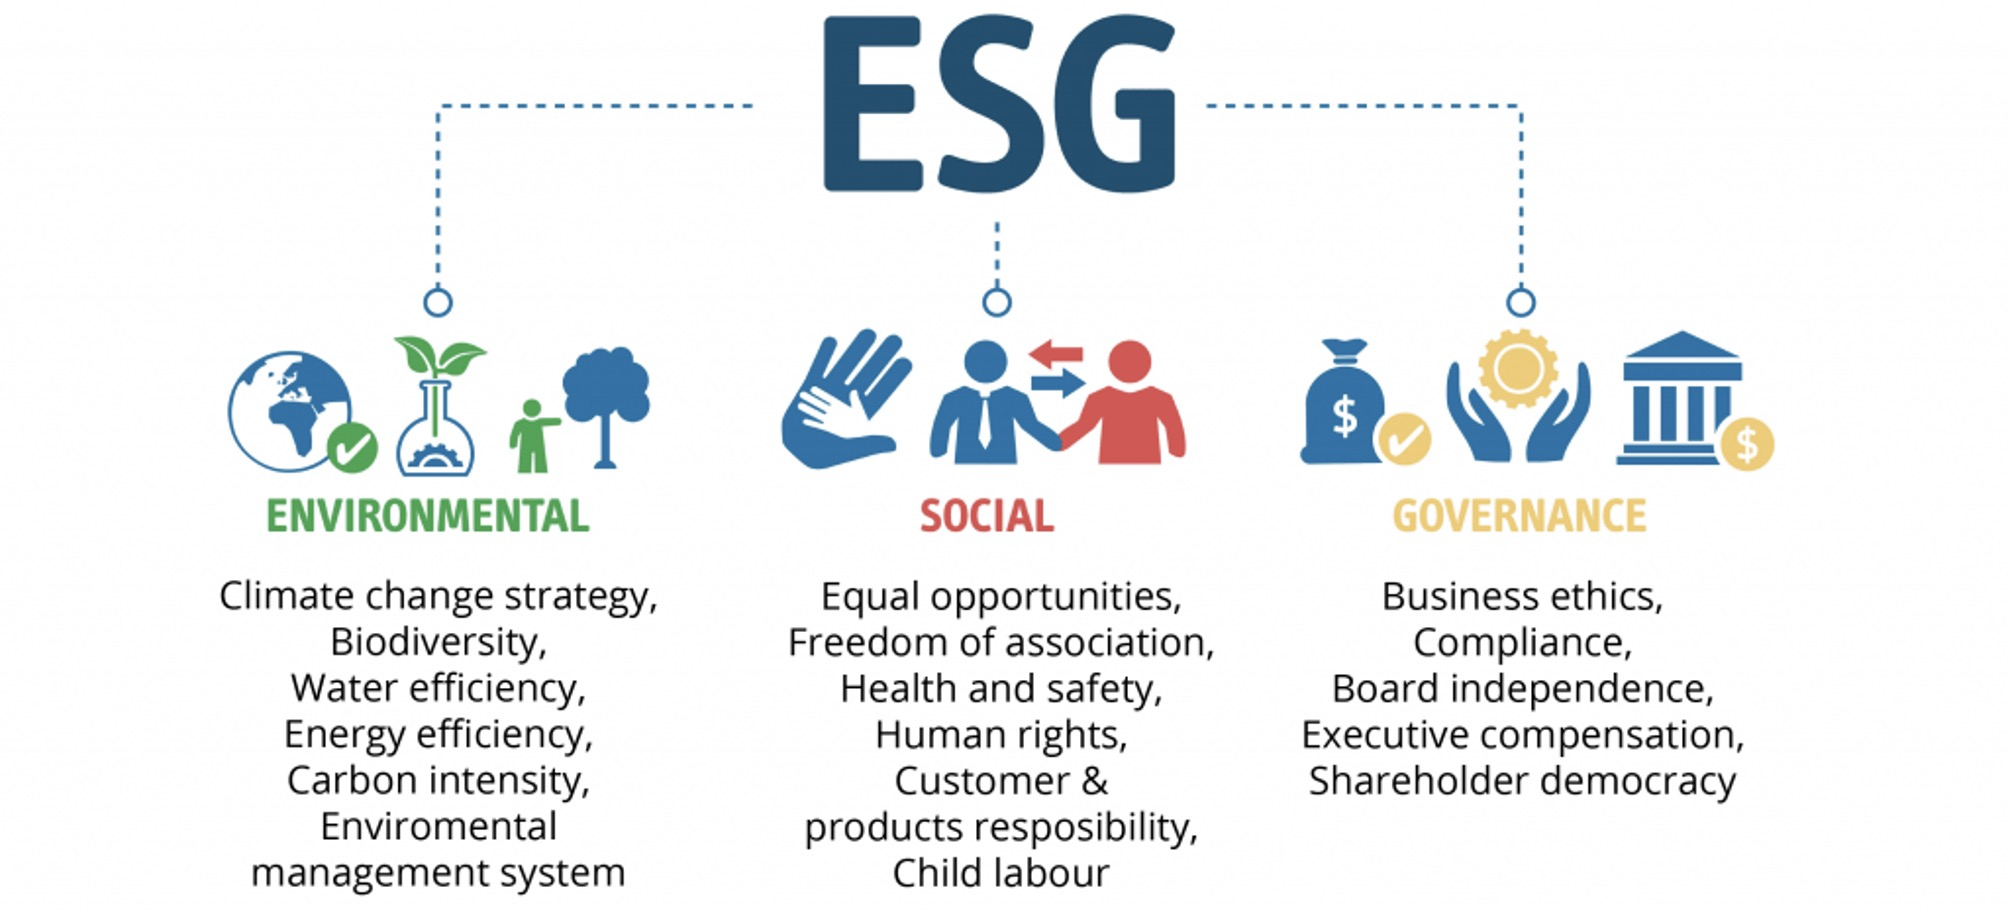
\includegraphics[width=0.6\linewidth]{./ESG} 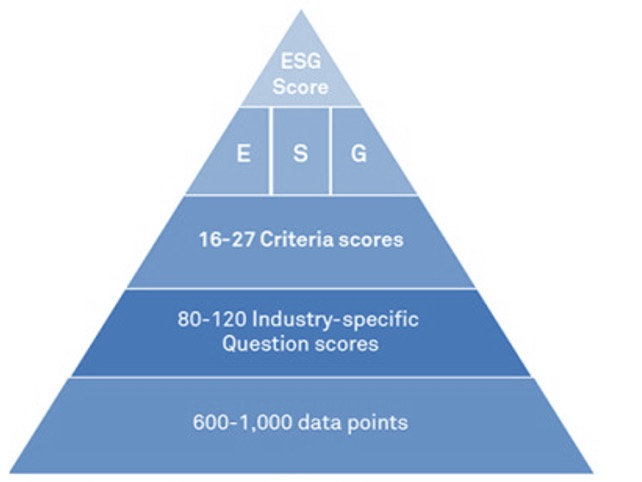
\includegraphics[width=0.35\linewidth]{./ESG Rating System} 

}

\caption{The Concept of ESG and ESG Rating System}\label{fig:ESG}
\end{figure}

Previous studies show that a firm's ESG profile and activities are
strongly related to the firm's market, leadership and owner
characteristics as well its risk, performance and value (Gillan et al.,
2021). Corporate ownership structures, as one of the indicators that
describe a company's identity, contribute to institutional oversight and
may affect companies' motives in promoting sustainability (Eng and Mak,
2003; Al Amosh \& Khatib, 2021). Even in front of the divergence of ESG
ratings due to distinctive scope, measurement, and weights (Berg et al.,
2019), what listed firms with great ESG performance look like is an
interesting question.

This paper investigates the ESG performance of publicly listed firms in
China during 2010-2020 and further explores the divergence of ESG
ratings, based on data from five prominent ESG rating agencies in China.
We finally apply a fixed-effect model to evaluate the association
between ESG scores and firm leadership and ownership characteristics.

We choose the following questions to guide our work:

\begin{itemize}
\tightlist
\item
  Are ESG scores from different rating agencies consistent without
  significant divergences?
\item
  How can these ownership structure factors (ownership concentration,
  blockholders' ownership, independent board ratio, chairman duality)
  affect ESG performance?
\end{itemize}

\newpage

\hypertarget{dataset-information}{%
\section{Dataset Information}\label{dataset-information}}

\hypertarget{data-retrieval}{%
\subsection{Data Retrieval:}\label{data-retrieval}}

For this analysis, we used data collected from Wind database including
basic characteristics, and financial statement information of 4912
listed firms during 2010-2021 in China. We also obtained ESG scores from
five ESG rating companies from their own databases: Sino-Securities
Index ESG, SynTao Green Finance ESG, China Alliance of Social Value
Investment (CASVI) ESG, FTSE Russell ESG, and Bloomberg ESG. Table 2
describes the sample size, rating and year ranges of the five ESG
indices. We downloaded these two excel files and added them to our
project repository. All data and code for this project can be retrieved
from the GitHub repository.

\begin{longtable}[]{@{}cccc@{}}
\caption{The Description of ESG Ratings}\tabularnewline
\toprule
ESG Index & Sample Size & Rating & Period \\
\midrule
\endfirsthead
\toprule
ESG Index & Sample Size & Rating & Period \\
\midrule
\endhead
Sino-Securities & 4065 firms & C, CC, CCC, B, BB, BBB, A, AA, AAA &
since 2009 \\
SynTao Green Finance & 765 firms & C-, C, C+, B-, B, B+, A-, A, A+ &
since 2015 \\
CASVI & 296 firms & C, CC, CCC, B, BB, BBB, A, AA, AAA & since 2016 \\
FTSE Russell & 728 firms & 0.3 - 3.9 & since 2018 \\
Bloomberg & 1122 firms & 6.6 - 64.1 & since 2010 \\
\bottomrule
\end{longtable}

\hypertarget{data-wrangling}{%
\subsection{Data Wrangling:}\label{data-wrangling}}

We began our analysis by transforming ESG ratings into numerical values.
Although two ESG ratings (FTSE Russell and Bloomberg) are numerical
values, the other three (Sino-Securities Index, SynTao Green Finance,
CASVI) are all rating levels. Thus, we regard these rating levels as
nine scores 1-9 from the lowest to the highest, for example, C equals 1,
CC equals 2, and so forth. Next, we applied many pipe functions with
\texttt{pivot\_longer} and created a date variable \texttt{Year} by
using \texttt{mutate} to adjust the structure of each data frame for
matching. Then, we merged one firm-characteristics dataset from Wind and
five ESG rating datasets by \texttt{stockcode} (stock ID) and
\texttt{Year} using \texttt{full\_join}. Finally, we obtained an unique
yearly firm-level panel dataset during 2010-2020.

For further analysis, we created new variables \texttt{Top1},
\texttt{Top25.Top1}, \texttt{IndepBoardRatio}, \texttt{ChairisGM} and
\texttt{StateOwned}. \texttt{Top1} equals the shareholding ratio of the
largest shareholder of a firm, which can measure the ownership
concentration; \texttt{Top25to1} equals to the ratio of the sum of
shares held by the \(2^{nd}\), \(3^{rd}\), \(4^{th}\), and \(5^{th}\)
largest shareholders to that of the \(1^{st}\) largest shareholder of a
firm, which can measure the blockholders' power;
\texttt{IndepBoardRatio} is the ratio of the number of independent board
members to the number of total board members, measuring board
independence; \texttt{ChairisGM} is a binary variable and equals 1 when
chairman and general manager (GM) are the same person, and 0 otherwise;
\texttt{StateOwned} is also a binary variable and equals 1 when a firm
is centrally or locally state-owned, and 0 otherwise. In addition, we
created several datasets for visualization and statistics.

\newpage

\hypertarget{exploratory-analysis}{%
\section{Exploratory Analysis}\label{exploratory-analysis}}

We conducted an exploratory analysis of our data visually using a
heatmap to show differences in ESG performance among the different types
of listed firms across years (Figure 2) and summary statistics tables to
provide an overview of basic characteristics of listed firms (Tables 2
and 3). The visualization showed that the average ESG score of listed
firms was increasing over the past ten years. Moreover, state-owned
firms and collective firms in China tend to constantly improve their ESG
performance with higher scores, while private firms and foreign firms
tend to be associated with decreasing and lower ESG scores during
2010-2020. It is worth mentioning that the average ESG score of foreign
listed firms in China decreased significantly in 2015, which might be
explained by the withdrawal of foreign capital and 2015 stock market
selloff. Details on the variables are available in the excel file on the
Github repository.

\begin{longtable}[]{@{}lrrrr@{}}
\caption{Summary Statistics for Firm-Level Variables}\tabularnewline
\toprule
Measure & \emph{Mean} & \emph{SD} & \emph{Max} & \emph{Min} \\
\midrule
\endfirsthead
\toprule
Measure & \emph{Mean} & \emph{SD} & \emph{Max} & \emph{Min} \\
\midrule
\endhead
ESG\_bloomberg & 22.524 & 5.730 & 64.115 & 9.091 \\
Environmental & 10.868 & 7.081 & 65.625 & 0.775 \\
Social & 25.431 & 8.725 & 77.193 & 3.509 \\
Goverance & 46.194 & 5.023 & 84.076 & 14.286 \\
ROA & 6.601 & 7.294 & 66.322 & -118.172 \\
ROE & 8.509 & 21.463 & 982.140 & -406.450 \\
Top1 & 39.427 & 16.202 & 93.673 & 3.390 \\
Top25to1 & 0.553 & 0.537 & 3.615 & 0.004 \\
ChairisGM & 0.145 & 0.352 & 1.000 & 0.000 \\
Size & 23.297 & 1.268 & 28.416 & 19.541 \\
LEV & 50.585 & 19.540 & 103.726 & 0.836 \\
CurrentRatio & 1.798 & 2.365 & 80.664 & 0.079 \\
IndepBoardRatio & 0.372 & 0.056 & 0.800 & 0.200 \\
StateOwned & 0.351 & 0.477 & 1.000 & 0.000 \\
\bottomrule
\end{longtable}

\begin{figure}
\centering
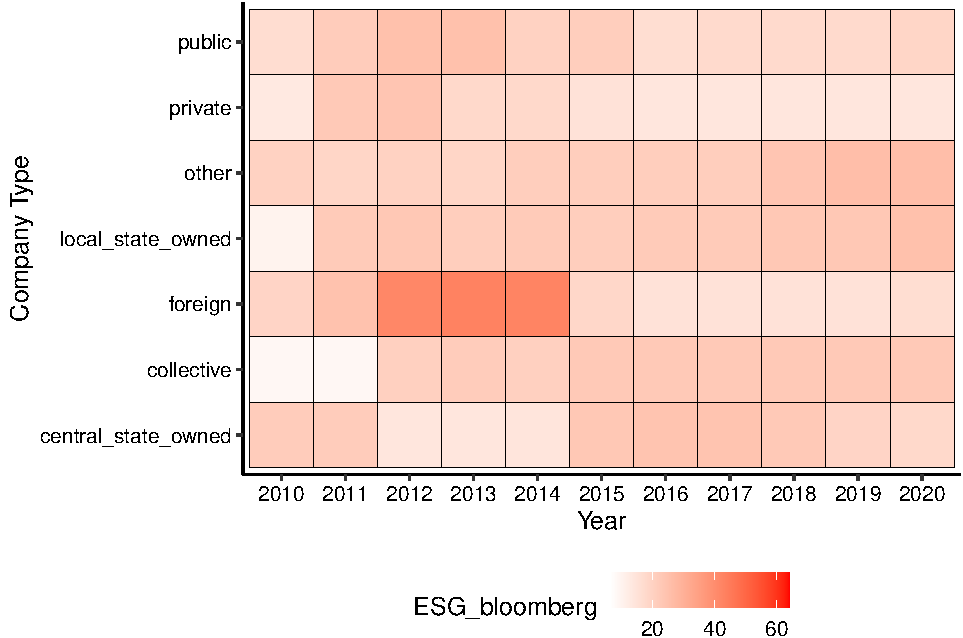
\includegraphics{FinalProject.Ruan.Muradov_files/figure-latex/heatmap-1.pdf}
\caption{Heat Map of ESG Rating of Different Types of Firms Across
Years}
\end{figure}

\begin{longtable}[]{@{}lrrrr@{}}
\caption{Bloomberg ESG Scores by Company Type}\tabularnewline
\toprule
Type & meanESG & minESG & maxESG & sdESG \\
\midrule
\endfirsthead
\toprule
Type & meanESG & minESG & maxESG & sdESG \\
\midrule
\endhead
central\_state\_owned & 22.318 & 6.612 & 51.240 & 6.770 \\
collective & 22.051 & 9.091 & 35.537 & 4.739 \\
foreign & 20.440 & 9.091 & 64.115 & 8.162 \\
local\_state\_owned & 20.835 & 7.438 & 52.066 & 6.290 \\
other & 19.340 & 11.157 & 29.752 & 3.815 \\
private & 19.229 & 7.438 & 60.744 & 6.279 \\
public & 21.882 & 8.678 & 53.719 & 7.955 \\
\bottomrule
\end{longtable}

\newpage

\hypertarget{analysis}{%
\section{Analysis}\label{analysis}}

\hypertarget{question-1-are-esg-scores-from-different-rating-agencies-consistent-without-significant-divergences}{%
\subsection{Question 1: Are ESG scores from different rating agencies
consistent without significant
divergences?}\label{question-1-are-esg-scores-from-different-rating-agencies-consistent-without-significant-divergences}}

Figure 3 and Table 4 show the correlation between ESG ratings. It is
clearly observed that all ESG ratings were positively correlated over
the past ten years, while the correlation coefficients were less than
0.60, not as high as we expected.

\begin{figure}
\centering
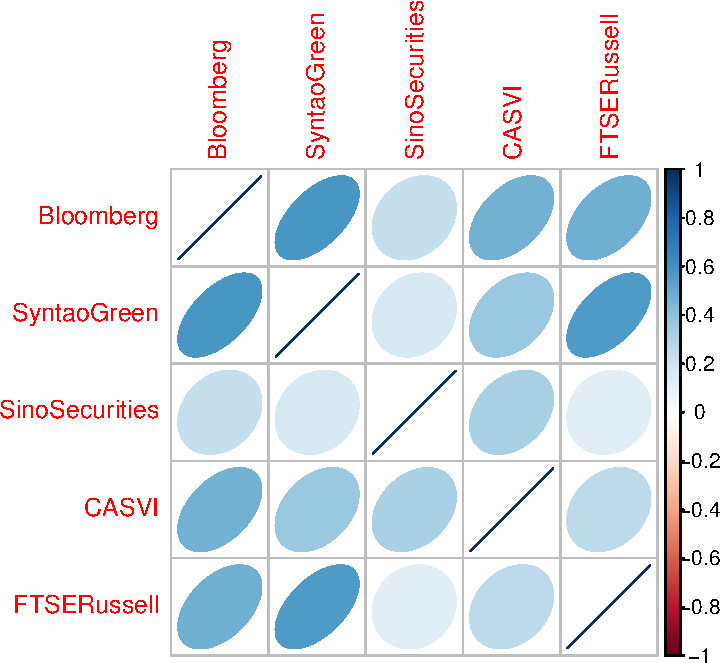
\includegraphics{FinalProject.Ruan.Muradov_files/figure-latex/ESG correlation-1.pdf}
\caption{The Correlation Plot for Five ESG Ratings}
\end{figure}

\begin{longtable}[]{@{}cccccc@{}}
\caption{The Correlation Table for ESG Ratings}\tabularnewline
\toprule
ESG Index & Bloomberg & SyntaoGreen & SinoSecurities & CASVI &
FTSERussell \\
\midrule
\endfirsthead
\toprule
ESG Index & Bloomberg & SyntaoGreen & SinoSecurities & CASVI &
FTSERussell \\
\midrule
\endhead
Bloomberg & 1.000 & 0.585 & 0.236 & 0.476 & 0.480 \\
SyntaoGreen & 0.585 & 1.000 & 0.178 & 0.375 & 0.561 \\
SinoSecurities & 0.236 & 0.178 & 1.000 & 0.321 & 0.122 \\
CASVI & 0.476 & 0.375 & 0.321 & 1.000 & 0.268 \\
FTSERussell & 0.480 & 0.562 & 0.122 & 0.268 & 1.000 \\
\bottomrule
\end{longtable}

Among these five ESG ratings, we should choose a reliable one for
further analysis. First of all, although Sino-Securities Index ESG
covers most of listed firms in China's stock market, including 4065 out
of 4912 listed companies, it has the lowest correlation coefficients
(less than 0.35) with other four indices. This means that its ESG rating
system is quite different from others. We exclude this one due to its
lower reliability. Furthermore, China Alliance of Social Value
Investment (CASVI) has a very small sample size, only including 296
listed companies after 2016, so we then exclude this one due to lack of
representativeness. Lastly, SynTao Green Finance, FTSE Russell, and
Bloomberg ESG indices are all highly positively correlated with darker
blue in Figure 3, which means their scope, measurement and weights are
consistent without many divergences. Since Bloomberg ESG includes 1122
listed firms during the period of 2010-2020 with fewer missing values
and is accurately measured by numerical scores rather than rating
levels, we choose Bloomberg ESG as a reliable index to measure ESG
performance of listed firms in China for further analysis.

\hypertarget{question-2-how-can-these-ownership-structure-and-leadership-factors-ownership-concentration-blockholders-ownership-independent-board-ratio-chairman-duality-affect-esg-performance}{%
\subsection{Question 2: How can these ownership structure and leadership
factors (ownership concentration, blockholders' ownership, independent
board ratio, chairman duality) affect ESG
performance?}\label{question-2-how-can-these-ownership-structure-and-leadership-factors-ownership-concentration-blockholders-ownership-independent-board-ratio-chairman-duality-affect-esg-performance}}

Figure 4 provides an overview of the relationship between ESG
performance of listed firms and four ownership structure and leadership
factors (ownership concentration, blockholders' power, board
independence, and chairman duality). Figure 5 also presents a
correlation plot to show associations between important variables.
However, simply measuring their relationships through correlation
coefficients and fitted lines are limited. Instead, we should apply a
multiple regression to further measure the effect of these four
ownership structure and leadership factors on ESG performance.

\begin{figure}
\centering
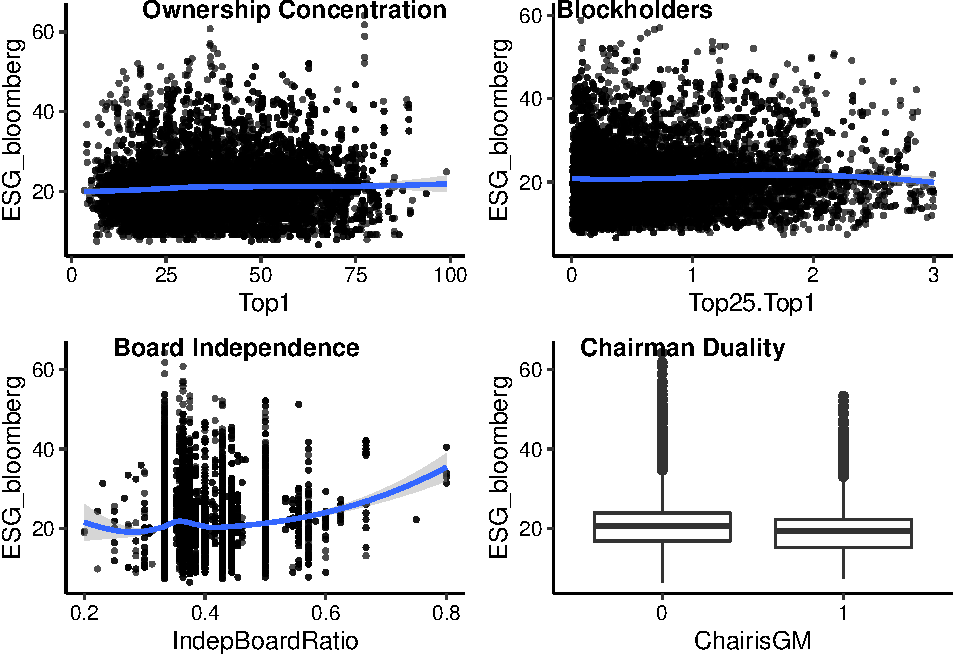
\includegraphics{FinalProject.Ruan.Muradov_files/figure-latex/plots-1.pdf}
\caption{Four Ownership Structure and Leadership Factors and ESG Rating}
\end{figure}

\begin{figure}
\centering
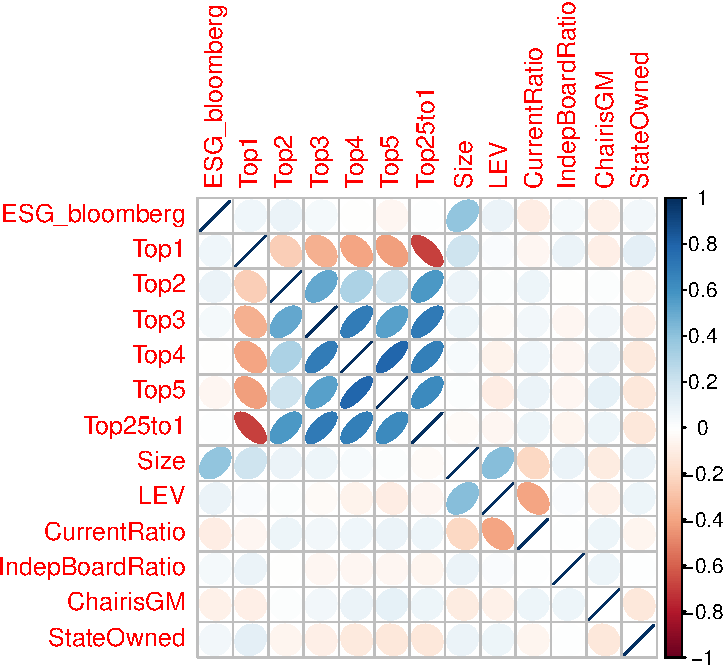
\includegraphics{FinalProject.Ruan.Muradov_files/figure-latex/correlation2-1.pdf}
\caption{The Correlation Plot for Important Variables}
\end{figure}

The regression equation is listed below. \begin{equation*}
\begin{split}
ESG_{it} = Top1_{it} + (Top1_{it})^2 + Top25to1_{it} + IndepBoardRatio_{it} + ChairisGM_{it} \\+ Size_{it} + LEV_{it} + CurrentRatio_{it} + \delta_t+\delta_j+\delta_{s}+\varepsilon_{it}
\end{split}
\end{equation*}

where \texttt{Top1} equals the shareholding ratio of the largest
shareholder of a firm; \texttt{Top25to1} equals to the ratio of the sum
of shares held by the \(2^{nd}\), \(3^{rd}\), \(4^{th}\), and \(5^{th}\)
largest shareholders to that of the \(1^{st}\) largest shareholder of a
firm; \texttt{IndepBoardRatio} is the ratio of the number of independent
board members to the number of total board members; \texttt{ChairisGM}
equals 1 when chairman and general manager (GM) are the same person, and
0 otherwise; \(\delta_t\), \(\delta_j\), and \(\delta_{s}\) represent
year fixed effect, industry fixed effect, and company type fixed effect;
\(\varepsilon_{it}\) is the unobserved error term.

Table 5 shows the regression result. Column (1) used all data during
2010-2020; Column (2) applied data during 2010-2014; and Column (3)
applied data during 2015-2020. By using Bloomberg ESG index for
regression, we find that 1) The higher ownership concentration is, the
higher ESG performance will be, but the marginal positive effect of
ownership concentration is decreasing; 2) The effects of outside
blockholders and independent board members are also significantly
positive at a 5\% level; 3) Chairman duality is not a good thing and
listed firm which chairman and general manager (GM) are the same person
tend to have lower ESG scores.

\begin{table}[!htbp] \centering \footnotesize
  \caption{Fixed-Effect Model} 
  \label{} 
\begin{tabular}{@{\extracolsep{5pt}}lccc} 
\\[-1.8ex]\hline 
\hline \\[-1.8ex] 
 & \multicolumn{3}{c}{\textit{Dependent variable:}} \\ 
\cline{2-4} 
\\[-1.8ex] & ESG2010-2020 & ESG2010-2014 & ESG2015-2020 \\ 
\\[-1.8ex] & (1) & (2) & (3)\\ 
\hline \\[-1.8ex] 
 Top1 & 0.088$^{***}$ & 0.088$^{***}$ & 0.085$^{***}$ \\ 
  & (0.016) & (0.022) & (0.022) \\ 
  & & & \\ 
 (Top1)$^2$ & $-$0.001$^{***}$ & $-$0.001$^{***}$ & $-$0.001$^{***}$ \\ 
  & (0.0002) & (0.0002) & (0.0002) \\ 
  & & & \\ 
 Top25to1 & 0.624$^{***}$ & 0.282 & 0.803$^{***}$ \\ 
  & (0.136) & (0.204) & (0.183) \\ 
  & & & \\ 
 Size & 1.916$^{***}$ & 1.781$^{***}$ & 2.044$^{***}$ \\ 
  & (0.049) & (0.072) & (0.067) \\ 
  & & & \\ 
 LEV & $-$0.027$^{***}$ & $-$0.034$^{***}$ & $-$0.022$^{***}$ \\ 
  & (0.003) & (0.004) & (0.005) \\ 
  & & & \\ 
 CurrentRatio & $-$0.107$^{***}$ & $-$0.096$^{***}$ & $-$0.155$^{***}$ \\ 
  & (0.017) & (0.018) & (0.034) \\ 
  & & & \\ 
 IndepBoardRatio & 2.494$^{***}$ & 4.356$^{***}$ & 0.637 \\ 
  & (0.908) & (1.296) & (1.240) \\ 
  & & & \\ 
 ChairisGM & $-$0.714$^{***}$ & $-$0.846$^{***}$ & $-$0.465$^{***}$ \\ 
  & (0.139) & (0.217) & (0.180) \\ 
  & & & \\ 
 ROA2 & $-$0.014$^{*}$ & $-$0.027$^{**}$ & $-$0.010 \\ 
  & (0.008) & (0.012) & (0.010) \\ 
  & & & \\ 
 Constant & $-$28.437$^{***}$ & $-$25.763$^{***}$ & $-$27.595$^{***}$ \\ 
  & (1.212) & (1.733) & (1.694) \\ 
  & & & \\ 
\hline \\[-1.8ex] 
Observations & 13,745 & 5,337 & 8,408 \\ 
R$^{2}$ & 0.280 & 0.255 & 0.258 \\ 
Adjusted R$^{2}$ & 0.275 & 0.243 & 0.250 \\ 
Residual Std. Error & 5.556 (df = 13649) & 5.012 (df = 5249) & 5.790 (df = 8317) \\ 
F Statistic & 55.879$^{***}$ (df = 95; 13649) & 20.664$^{***}$ (df = 87; 5249) & 32.064$^{***}$ (df = 90; 8317) \\ 
\hline 
\hline \\[-1.8ex] 
\textit{Note:}  & \multicolumn{3}{r}{$^{*}$p$<$0.1; $^{**}$p$<$0.05; $^{***}$p$<$0.01} \\ 
\end{tabular} 
\end{table}

\newpage

\hypertarget{summary-and-conclusions}{%
\section{Summary and Conclusions}\label{summary-and-conclusions}}

\hypertarget{increasing-trend}{%
\subsection{Increasing Trend}\label{increasing-trend}}

Overall, although the average ESG score of listed firms in China was
only 22.524, relatively lower compared to U.S. firms, these listed firms
have been working hard on improving ESG performance over the past ten
years. Specifically, state-owned firms and collective firms in China
tend to constantly improve their ESG performance with higher scores,
while private firms and foreign firms tend to be associated with
decreasing and lower ESG scores during 2010-2020. Interestingly, the
average ESG score of foreign listed firms in China decreased
significantly in 2015, which might be explained by the withdrawal of
foreign capital and 2015 stock market selloff.

\hypertarget{esg-divergence-and-selection}{%
\subsection{ESG Divergence and
Selection}\label{esg-divergence-and-selection}}

Globally, different ESG rating agencies have common differences in the
ESG ratings of a company. The divergence can be decomposed into
contributions of scope, measurement, and weights (Berg et al., 2019).
The ESG ratings from five main rating companies in China were all
positively correlated, but still had significant divergence.
Sino-Securities Index ESG covers 4065 listed companies, but has the
lowest correlation coefficients with other four indices. China Alliance
of Social Value Investment (CASVI) only includes 296 listed companies
after 2016, so the sample size is not large enough to be representative.
SynTao Green Finance, FTSE Russell, and Bloomberg ESG indices are all
highly positively correlated, but Bloomberg ESG has fewest missing
values and is directly measured by numerical scores rather than rating
levels. Therefore, we choose Bloomberg ESG as a reliable index to
measure ESG performance of listed firms in China for our analysis.

\hypertarget{ownership-structure-and-leadership-factors}{%
\subsection{Ownership Structure and Leadership
Factors}\label{ownership-structure-and-leadership-factors}}

Based on our analysis, ownership concentration is beneficial for
improving ESG performance to some extent, but the marginal effect is
decreasing. This may indicate that the largest shareholder with more
shares help stabilize the corporate governance and apply sustainable and
consistent strategy, while one person with too much power is more likely
to be autarchic, leading a corporate to a wrong direction more easily.
The effects of blockholders and independent board members on ESG
performance are also significantly positive. This may show that
democracy and independence are essential to make rational decisions and
avoid corruption. Lastly, chairman duality is not a good choice and
listed firm should try to make sure that chairman and general manager
are not the same person.

\hypertarget{future-recommendations}{%
\subsection{Future Recommendations}\label{future-recommendations}}

Even in Europe today, only 30\% of the largest publicly traded
corporations fully disclose their business model's environmental and
climate-related implications (CDSB, 2020). It goes without saying that
the topic of ESG is relatively new in the world and the reports like
ours concentrating on the identification of factors for construction of
ESG policies and strategies would not be as reliable as it will be in
15-20 years, considering the changing politics. That effectively means
the research area and data on ESG will improve throughout time and
indicators might undergo refreshments and modifications. Additionally it
is important to consider the cultural factors that could affect ESG
performance of the companies on top of the factors such as corruption
nepotism size of the company and others that we have explored to be able
to capture the model in a broader way, account for more variabilities
and, thus, achieve greater level of \(R^2\). Another issue could be
addressed such as the political stability in the country which is
actually one of the central tenets of creditworthiness in the business
world. As we know it most of the credit lenders and investors are today
moving to hunt those companies with higher ESG performance levels and
this is one of the greatest priorities for their companies to achieve
greater levels of ESG score for attracting more financing opportunities.
However, ESG levels are not the most important factors in the are
influencing investor decisions and external factors like the value of a
local currency could be explored in deeper perspective in order to shed
light on the mutual interplay between ESG and creditworthiness to assist
those companies as well as the governments in understanding how to
regulate their balance of payments to bring about net positive ESG
performance levels in the local companies.

\newpage

\hypertarget{references}{%
\section{References}\label{references}}

Al Amosh, H., \& Khatib, S. F. A. (2021). Ownership structure and
environmental, social and governance performance disclosure: The
moderating role of the board independence. Journal of Business and
Socio-Economic Development, ahead-of-print(ahead-of-print).
\url{https://doi.org/10.1108/JBSED-07-2021-0094}

Berg, F., Kölbel, J. F., \& Rigobon, R. (2019). Aggregate Confusion: The
Divergence of ESG Ratings (SSRN Scholarly Paper No.~3438533). Social
Science Research Network. \url{https://doi.org/10.2139/ssrn.3438533}

Bloomberg NEF. (2022). Energy Transition Investment Trends 2022.
Retrieved on April 7th 2022, from
\url{https://assets.bbhub.io/professional/sites/24/Energy-Transition-Investment-Trends-Exec-Summary-2022.pdf}

CDSB (2020). Falling short? Climate Disclosure Standards Board.
Retrieved April 20, 2022, from \url{https://www.cdsb.net/falling-short}

Eng, L.L. and Mak, Y.T. (2003), ``Corporate governance and voluntary
disclosure'', Journal of Accounting and Public Policy, Vol. 22 No.~4,
pp.~325-345.

Freeman, R. E. (1984). Strategic management: A stakeholder theory.
Journal of Management Studies, 39(1), 1-21.

Gillan, S. L., Koch, A., \& Starks, L. T. (2021). Firms and social
responsibility: A review of ESG and CSR research in corporate finance.
Journal of Corporate Finance, 66, 101889.
\url{https://doi.org/10.1016/j.jcorpfin.2021.101889}

\end{document}
